\documentclass[problem]{mcs}

\begin{pcomments}
    \pcomment{TP_The_Divisibility_DAG}
    \pcomment{Converted from divides-dag.scm
              by scmtotex and dmj
              on Sun 13 Jun 2010 02:58:06 PM EDT}
\end{pcomments}

\begin{problem}

%% type: short-answer
%% title: The Divisibility DAG

\begin{center}
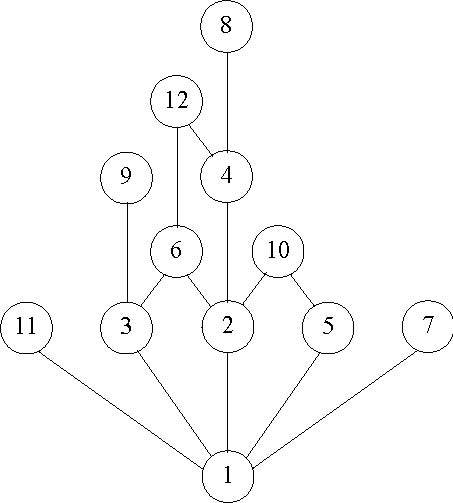
\includegraphics{divi2}
\end{center}

In this~\ref{???} DAG for the divisibility relation on $\{1, \dots,
12\}$, there is an upward path from $a$ to~$b$ iff $a | b$.  If 24 was
added as a vertex, what is the minimum number of edges that must be
added to the DAG to represent divisibility on $\{1, \dots, 12, 24\}$?

\begin{solution}
2

Edges from 8 and 12 to 24 are all that are needed.
\end{solution}

\end{problem}

\endinput
